\documentclass[12pt]{article}

% House style preamble
\input{.house-style/preamble.tex}

% Update PDF metadata
\hypersetup{
  pdftitle={Normative Status in Causal Networks}
}
\AtBeginBibliography{\emergencystretch=3em\sloppy}

% PROVISIONAL TITLE. Candidates under consideration (see planning/brief.md):
%   - What Is a Causal-Normative Network?            (blunt)
%   - Normative Status in Causal Networks            (journal-friendly; current pick)
%   - How Normative Status Enters Causal Explanation (journal-friendly)
%   - Mixed Networks: Causation, Recognition, and Deontic Status
%   - The Structure of Causal-Normative Explanation
\title{Normative Status in Causal Networks}
\author{Brett Reynolds \orcidlink{0000-0003-0073-7195}%
\thanks{Contact: \href{mailto:brett.reynolds@humber.ca}{brett.reynolds@humber.ca}}\\
Humber Polytechnic \& University of Toronto}
\date{\today}

% Typed-edge network diagrams (local figure support)
\usepackage{tikz}
\usetikzlibrary{arrows.meta, positioning}
\definecolor{xGreen}{RGB}{27,158,119}
\definecolor{xOrange}{RGB}{217,95,2}
\definecolor{xPurple}{RGB}{117,112,179}
\newcommand{\Nd}[2]{\textsf{\footnotesize #1:}\\#2}
\tikzset{
  kind/.style={draw, rounded corners, align=center, font=\small, inner sep=3pt, minimum height=9mm},
  ghost/.style={draw, rounded corners, align=center, font=\small, inner sep=3pt, minimum height=9mm,
                draw=gray, text=gray, dash pattern=on 2pt off 1.5pt},
  flagged/.style={draw, rounded corners, align=center, font=\small, inner sep=3pt, minimum height=9mm,
                draw=black, text=black, dash pattern=on 3pt off 2pt},
  causal/.style={-{Stealth}, semithick},
  ntrans/.style={-{Triangle}, semithick, xOrange},
  constit/.style={xPurple, very thick, double, double distance=1pt},
  recog/.style={-{Stealth}, semithick, dashed, xGreen},
  void/.style={gray, very thick, double, double distance=1pt, dash pattern=on 2pt off 2pt},
}
\newcommand{\edgelegend}{%
  \begin{scope}[shift={(0,-3.4)}]
    \draw[causal] (0,0) -- ++(0.9,0);    \node[right,font=\footnotesize] at (1.0,0) {causal};
    \draw[constit] (0,-0.6) -- ++(0.9,0); \node[right,font=\footnotesize] at (1.0,-0.6) {constitutive};
    \draw[ntrans] (5.2,0) -- ++(0.9,0);   \node[right,font=\footnotesize] at (6.2,0) {normative-transition};
    \draw[recog] (5.2,-0.6) -- ++(0.9,0); \node[right,font=\footnotesize] at (6.2,-0.6) {recognitional};
  \end{scope}%
}

\begin{document}
\maketitle

\begin{abstract}
Some social and moral explanations need causal relations and normative transitions in one structure. I call that structure a \term{causal-normative network}: statuses alter practical positions, causal mechanisms transmit uptake and response, and recognition links let agents and institutions track, mis-track, or alter statuses. Extending \textcite{khalidi2018nodes}'s account of projectible kinds as ordered nodes in causal networks, I argue that moral and institutional cases require four dependence types: causal, constitutive, normative-transition, and recognitional. Misrecognition is diagnostic, because it shows how a status-assignment can become socially effective, and sometimes valid within a field, without acquiring moral warrant.
% TODO: tighten to journal abstract length once §§4--6 stabilise.
\end{abstract}

\section{The problem of mixed explanation}
\label{sec:problem}

Suppose a community comes to treat someone as having promised when he hasn't, or as bound by a debt he never incurred. The treatment is entirely real: he is asked to pay, blamed when he refuses, distrusted, perhaps shut out. But he's under no obligation. The demand has the social force of a warranted demand and none of its warrant. A status-assignment, it seems, can be socially effective without the standing it claims, and explaining how that's possible is the problem of this paper.

Two tidy answers fail. Say the status just is the treatment, what people do, and the wrongly-hounded man becomes indistinguishable from a genuine debtor: warrant drops out. Say the status is a normative fact fixed by the rules and indifferent to what anyone does, and the treatment becomes mere noise: the efficacy drops out. But the phenomenon needs both, a normative position and a causal take-up that can fit it or fail to. So the animating question is what kind of explanatory structure holds causal relations and normative transitions together without reducing either to the other.

Promising is the case I work through, because its life-cycle is familiar and its parts are clean: an act creates an obligation, the obligation is recognized and relied on, breach sets off demand and repair, release cancels the profile. And the same shape recurs in consent, in official judgment, and, most systematically, in discrimination, where an assignment that's effective, and even valid within its field, hardens into a regime that morality disowns (Section~\ref{sec:misrecognition}). I keep to promising until then.

The apparatus rests on four kinds of dependence, three of them directed edges and the fourth a non-directed constitutive tie.

First, \term{causal dependence}: one event, disposition, procedure, response, record, sanction, or expectation helps produce another. A public promise causes reliance; a judgment causes enforcement; a recognition state causally drives treatment, and that uptake is where much of the network's efficacy lies.

Second, \term{constitutive dependence}: one deontic position is the correlative of another within a single complex. A duty and the claim-right held against the duty-bearer are one jural relation under two descriptions, so from either one reads off the other \citep{hohfeld1913SomeFundamental}. The tie is constitutive, not causal.

Third, \term{normative-transition dependence}: a performance, rule, status, or transition event generates, blocks, terminates, defeats, or modifies a status. An undertaking generates a duty; release terminates it; withdrawal terminates a permission; breach generates a secondary profile of demand, blame, apology, repair, or excuse.

Fourth, \term{recognitional dependence}: a belief, record, uptake, or official classification tracks a status, fitting or failing to fit it. But what recognition then drives is causal uptake: demand, sanction, reliance, exclusion. Where recognition is authorized to make the status it records, as a court judgment makes a liability, the case is compound, not a fifth primitive.

\section{Why ordinary causal networks aren't enough}
\label{sec:causal-not-enough}

Start with the best version of the causal picture. \textcite{khalidi2018nodes} argues that a kind is projectible not because its properties happen to co-occur but because they're causally ordered: a few core properties cause a cascade of derivative ones, and the kind shows up as a highly connected node in a directed causal graph, its edges read in interventionist terms, so that one property is a direct cause of another when intervening on the first shifts the second with the rest held fixed.

Order, not concatenation, is what supports projection. A heap of co-occurring properties (Khalidi's functionless widget) licenses nothing; an ordered network licenses inference along its edges. This is right, and the account here keeps it.

The work is done by directedness. Because the edges run one way, we can project: from core to derivative, and, more cautiously, back. Khalidi is careful about the social domain. Some social categories, senior citizen or felon, cluster by legislative fiat rather than causality and so aren't projectible kinds; others, refugee or consumer, earn kindhood because their properties are causally linked.

Convention either defeats projectibility or, where a conventional category comes to play a causal role, matters only by feeding into causal structure. But Khalidi never allows an edge that's neither causal nor a defect while carrying projectible order in its own right.

That is exactly what the moral and institutional cases need. Take the promise of Figure~\ref{fig:promise}. The duty and the promisee's claim-right are correlative, one relation under two descriptions, so the structure here is real but not causal: neither position is an effect of the other.

And transition orders the network too. The same non-performance counts as a breach before release and not after, but release causes nothing in Khalidi's sense; it changes what the later act amounts to. That dependence is directed and supports projection, from a breach one projects to liability or repair, but it isn't causal.

So the pivot. Khalidi is right that projectibility requires order; the moral and institutional cases show that not all order is causal order. The lesson is not to abandon his framework but to widen the notion of order it rests on.

What grounds projection is directed dependence, and causal dependence is one species of it, alongside the normative-transition and recognitional dependences just seen; these directed edges run within constitutive constraints that fix the deontic positions they connect. Projection runs along the directed edges whatever their type. Section~\ref{sec:typed-edge} builds the resulting typed network; the present point is only that ordinary causal networks are too narrow, not that order was the wrong demand.

\section{Why normative taxonomies aren't enough}
\label{sec:normative-not-enough}

Now the opposite simplification. The normative structure is real, and analytic jurisprudence has mapped it well: \textcite{hohfeld1913SomeFundamental} sorts deontic positions into correlatives and opposites, claim and duty, power and liability, and a taxonomy in this style can say that a promise generates an obligation, consent a permission, release a termination, and breach a license to complain. None of this is wrong. But the question is whether it's enough to explain why such classifications are projectible.

It isn't, because projectibility is a fact about practice, not entailment. A taxonomy tells us what follows normatively from a breach; it doesn't tell us that the breach is noticed, that complaint is made and taken up, that the promisor apologizes or excuses, that repair or sanction follows, and that trust is revised. And those are the regularities we actually project from promise-breaking; they run through recognition and causal uptake, not through the deontic entailment alone.

The promise-breaking life-cycle makes this concrete.
% TODO: cite the act-kinds sister paper's promise-breaking life-cycle once it is posted.
A breach sets off a recognitional and causal cascade: the promisee registers it, demands or blames; the promisor apologizes or offers an excuse; repair or sanction follows; trust is revised. The kind is projectible because acts occupy stable positions in that cascade, above and beyond meeting the definition of breach.

The status is thus necessary but not sufficient. A status no one could recognize, rely on, or enforce would support no projection at all, which is just the well-formedness condition of Section~\ref{sec:typed-edge}: a status does projectible work only where response states are reachable from it through recognition and causal uptake.

This is the mirror of Section~\ref{sec:causal-not-enough}. There, causal order alone was too narrow; here, normative order alone is too thin. A bare deontic taxonomy is, in Khalidi's sense, a list of co-occurring normative properties with no projectible cascade \citep{khalidi2018nodes}; it earns projectibility only once embedded in uptake and response. Together the two sections close off the forced choice from both sides: the explanatory unit is neither causal regularity nor normative status, but a normative position coupled to causal uptake. Where the two come apart is the business of Section~\ref{sec:misrecognition}.

\section{The typed-edge model}
\label{sec:typed-edge}

A causal-normative network has different kinds of node and, more to the point, different kinds of edge. The heterogeneity is the point, not a defect to be explained away.

I keep \textcite{khalidi2018nodes}'s picture of a kind as a highly connected node in a directed graph, but I let the edges differ in type. The vertices are property instances and states; the edges are typed relations of dependence.\footnote{Formally, this is a typed-edge relational structure: node labels for kinds, edge labels for dependence types, with well-formed cases fixed by constraints on configurations. In a formal treatment of English syntax, \textcite{pullumRogers2008Expressive} use node-labelled categories and edge-labelled functions. Nothing in the argument depends on the analogy; it only marks the intended level of formal abstraction. \textcite{pullum2001} set out the model-theoretic stance.}

What changes is that not every edge is a relation of direct causation.

The nodes include performances (utterances, signatures, actions, omissions), deontic statuses (obligation, permission, power, liability, immunity, standing), transition events (undertaking, authorization, release, withdrawal, breach, defeat), recognition states (belief, record, official classification, uptake), response states (blame, resentment, apology, repair, sanction, trust update), and field structures (legal, interpersonal, institutional, professional, medical, epistemic).

Three of the four dependences are directed edges, causal, normative-transition, and recognitional; the fourth, the constitutive tie, is a non-directed correlative. Two further notions are often mistaken for primitive edges but aren't. \emph{Authorized recognition} (a court judgment that makes the liability it records) is a compound of a recognitional and a transition edge. \emph{Projection} (a classification licensing defeasible inferences about later states) isn't a dependence in the network at all; it's the inferential use we make of one.

The edge types are told apart by how they behave under intervention. \textcite{woodward2003MakingThingsHappen} counts a relation as causal when some possible intervention on the first variable changes the second while everything else is held fixed, and the change reaches the second only through the first \citep{woodward2014MethodologyOntology}. A causal edge passes this test: intervene on the utterance and reliance shifts, intervene on the judgment and enforcement follows. Khalidi already reads his own causal edges this way \citep{khalidi2018nodes}, which is why typing the edges extends his picture rather than breaking with it.

A constitutive tie fails the test, and fails it diagnostically. A duty and its correlative claim-right aren't two states linked by a mechanism; they're one jural relation under two descriptions \citep{hohfeld1913SomeFundamental}. No intervention changes the duty while holding the claim-right fixed, because changing the one just is changing the other: the change doesn't reach the claim-right only through the duty, it lands on both at once. By Woodward's own criterion the tie therefore isn't causal, and that failure is what marks it as constitutive.

The transition and recognitional edges are directed without being causal. A normative-transition edge runs from a performance, rule, status, or transition event to the status it generates, terminates, blocks, defeats, or modifies: release the promisor and the same non-performance is no longer a breach.

A recognitional edge links a status to a recognition that tracks it, but the recognition can fit, mis-fit, or have no status to track at all, and that gap is what the \enquote{mis-} in misrecognition marks. Whether it fits is a separate question from what it then sets off, since the uptake from a recognition state to treatment, demand, sanction, reliance, exclusion, is itself causal: it's the point where the normative layer re-enters the causal one.

An illocutionary act, in \textcite{sbisa2023OnIllocutionaryTypes}'s terms, assigns or cancels deontic-modal predicates, and so appears here as a performance feeding a normative-transition edge.

Figure~\ref{fig:promise} renders a promise as a small network of this kind, with the four edge types that recur across the carrying cases.

\begin{figure}[tb]
  \centering
  \resizebox{\textwidth}{!}{%
  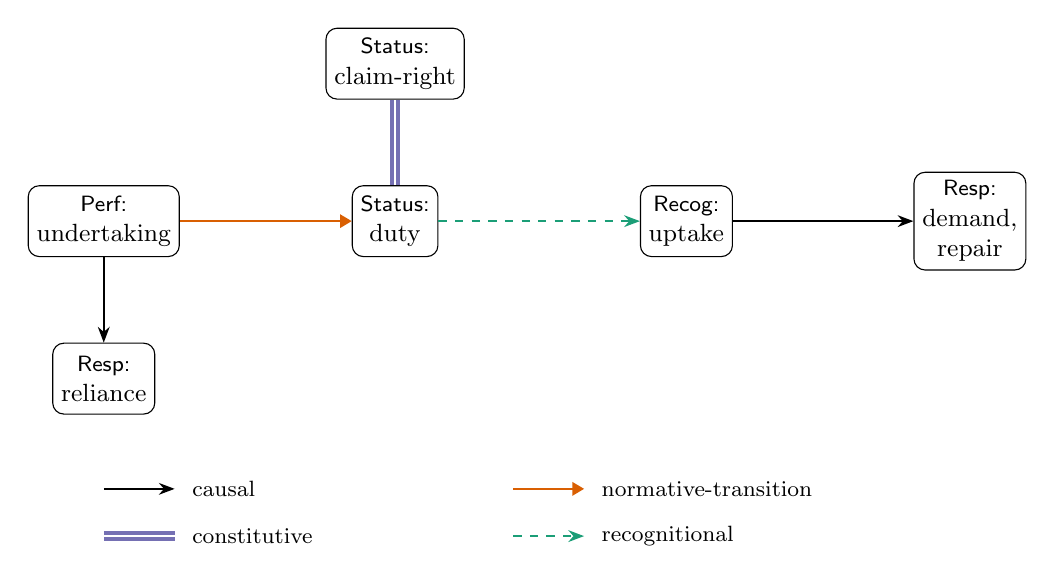
\begin{tikzpicture}
    \node[kind] (u) at (0,0)    {\Nd{Perf}{undertaking}};
    \node[kind] (o) at (3.7,0)  {\Nd{Status}{duty}};
    \node[kind] (k) at (3.7,2)  {\Nd{Status}{claim-right}};
    \node[kind] (r) at (7.4,0)  {\Nd{Recog}{uptake}};
    \node[kind] (d) at (11.0,0) {\Nd{Resp}{demand,\\repair}};
    \node[kind] (l) at (0,-2)   {\Nd{Resp}{reliance}};
    \draw[ntrans]  (u) -- (o);
    \draw[recog]   (o) -- (r);
    \draw[causal]  (r) -- (d);
    \draw[constit] (o) -- (k);
    \draw[causal]  (u) -- (l);
    \edgelegend
  \end{tikzpicture}}
  \caption{A promise as a causal-normative network. The undertaking generates the duty (a normative transition) and causally induces reliance; the duty carries its correlative claim-right (a constitutive tie, drawn without an arrowhead, since correlatives are one relation under two descriptions, not a directed cause); the duty is tracked by recognition, whose uptake causally drives demand and repair. The four edge types are keyed below the graph.}
  \label{fig:promise}
\end{figure}

Two conditions keep such a graph from sliding back into a mere list of properties. First, inference has to respect edge type: one may project enforcement from a judgment along a causal edge, or a claim-right from a duty across a constitutive tie, but not treat the second as though it were the first. Second, every status that figures in explanation has to be reachable by response states through recognition and its causal uptake; a status that could not be recognized or taken up within any practice explains no projectible social cascade (the argument of Section~\ref{sec:normative-not-enough}).

With those conditions in place the graph carries order in Khalidi's sense, projection along directed edges, while generalizing what that order is: not causal dependence throughout, but directed dependence of three kinds, causal, normative-transition, and recognitional, running within constitutive constraints.

All these nodes and edges are field-indexed: which performances count, which recognitions are authoritative, and which responses are licensed depends on the field, to which Section~\ref{sec:fields} returns.

\section{Coupling and counterfactual signatures}
\label{sec:coupling}

What makes this one network rather than a causal system with a normative commentary bolted on? The edges are coupled: a change to one type propagates through the others in patterned, counterfactually stable ways, and the pattern depends on which type you perturb. Three counterfactual signatures make the coupling visible, because each fixes what moves and what holds. But I reserve \emph{intervention} for the genuinely causal edges, where Woodward's apparatus applies directly, and call these typed contrasts \emph{signatures}.

A \term{status-rule signature}: change a status or the rule that governs it, a normative transition. The deontic profile changes, and uptake changes downstream (the order is explanatory, not temporal). Release the promisor and the same non-performance stops being a breach, so the demand, blame, and repair that breach would license lapse with it. Withdraw consent and the same touching becomes a trespass. Speak without standing and the same words fail to bind. These are the status-altering acts the normative-powers literature describes \citep{owens2012ShapingNormativeLandscape,raz2022NormativePowers}.

A \term{recognition signature}: change the recognition that tracks a status while the status itself holds fixed. Now recognition and its causal downstream move, but the underlying status doesn't. A person falsely believed to have promised meets demand, blame, and withdrawn trust he doesn't owe; a valid consent that goes unrecognized fails to protect. Woodward's own reading of \enquote{being a woman causes hiring discrimination} relocates the cause to the employer's beliefs about the applicant's gender \citep{woodward2014MethodologyOntology}: a recognition signature in the present sense, capturing the efficacy and saying nothing about warrant.

An \term{authorized recognition} signature changes an authorized recognition, the compound that's recognitional and status-altering at once, so recognition and status move together. A judgment creates the liability, a registration creates the record that counts, an accepted resignation ends the office \citep{americanLawInstitute1981RestatementContracts}. Here recognition doesn't track a status it finds already in place; the practice has given the recognizing act the power to make the status it records.

But no fourth type answers to constitutive edges: those show up as the failure of surgical intervention (Section~\ref{sec:typed-edge}), not as a signature of their own. I also set aside the pure causal intervention, severing an uptake mechanism so the letter never arrives, because both reductive views already grant it and it can't tell them apart from the coupled account.

The three that matter touch status and recognition, which is just where the forced choice goes wrong. The recognition-only reduction predicts that enough recognition constitutes the status, collapsing the recognition signature into a status change; the normative reduction predicts that recognition without a status change is mere noise, denying its efficacy. The recognition signature refutes both, and Section~\ref{sec:misrecognition} builds on it.

So the coupling claim can be put sharply. From which edge a probe perturbs, one can predict which of status and uptake will move and which will hold, and the prediction is stable across the carrying cases. A causal graph with moral labels can't deliver the status-rule signature, since labels don't propagate; a normative taxonomy with sociology appended can't deliver the recognition signature, since it has nowhere to put efficacy without warrant. Only the coupled, typed structure gets all three right at once, and that joint stability is what makes it one network.

A last objection runs the other way. An interventionist may say that \term{causal-normative network} merely relabels several ordinary causal variables imprecisely, and should be disambiguated into manipulations of beliefs, records, and behavior. But the reply turns on Woodward's own view that interventionism is methodology, not ontology \citep{woodward2014MethodologyOntology}: it clarifies causal claims by tying them to hypothetical experiments, and is explicitly non-reductive.

Typing edges by their signatures therefore reduces nothing; it shows that the hypothetical experiments come in different kinds, and that two of them need a status variable no bookkeeping over beliefs and behavior recovers. The interventionist's own disambiguation of the discrimination case relocates the cause to a belief and so drops the question whether the belief is correct, which is the normative question. The framework meant to dissolve the network instead marks the point where the normative edge is required.

\section{Misrecognition as the diagnostic case}
\label{sec:misrecognition}

Misrecognition is the sharpest diagnostic, because it forces both reductions to misdescribe a familiar phenomenon. On the recognition-only reduction, enough uptake would constitute the status: if everyone treats me as having promised, then I have promised, and a status is just its recognitional and causal trace. On the normative reduction, the causal effects of a mistaken or imposed status are mere noise around a normative fact that holds wherever the rules put it. But both are wrong. A misrecognized status can be causally powerful and morally void at once.

The apparatus separates things the reductions run together. A status-assignment is socially effective when its recognitional and causal edges fire: agents and institutions take it to hold, and rely, demand, enforce, exclude, and record accordingly. And it's field-valid when the status-generating conditions of that field are actually met.

Validity itself isn't a single thing: an assignment can be valid by the rules of its field, the right party, the right form, the right record, but morally void; or morally grounded but recognized by no institution. Efficacy is one thing, field-validity a second, moral warrant a third, and they can come apart. The effective-but-morally-void case is the one that matters (Figure~\ref{fig:misrecognition}).

An assignment that fails the conditions it purports to satisfy is still a structure, not noise: that's what lets misrecognition be real in its effects without being correct, and it grades the defect. A person wrongly believed to have promised is a local, corrigible failure; a durable regime entrenches the misfit across many nodes, with its own authority-like uptake.

What kind of structure? Ásta's conferralist account gives one: a social status is conferred on a person because others take them to have some base property, whether or not they actually have it, and the status consists in real constraints and enablements on what they may do \citep{asta2018Categories}. The ascribed standing is thus not a mere belief but a conferred social position with teeth.

Conferralism can look like a threat here: if the status just is what gets conferred, then enough recognition does constitute it, and the effective-without-warrant case collapses. But the threat dissolves once validity is typed. Conferral constitutes a social status, real within its community and fully effective, but it confers no moral warrant. A discriminatory standing is at once genuinely conferred and genuinely baseless, real in one sense and void in another.

Two cases should be kept apart, then. In \emph{local misrecognition} the recognition fails to fit a status that isn't there, the wrongly-hounded debtor of Section~\ref{sec:problem}. In \emph{wrongful conferral} the recognition does produce a status, real and perhaps field-valid, that lacks moral warrant, the discriminatory standing. The first is a tracking failure, the second a morally baseless success; both are diagnostic, for opposite reasons.

Some oppressive regimes work through stabilized wrongful conferral, where morally indefensible status-ascriptions become socially effective, and often field-valid, along durable recognition and response pathways. Not all oppression is like this; much is material, distributive, or coercive, not a matter of recognition at all, the pressure the redistribution-versus-recognition debate brings to bear \citep{fraserHonneth2003Redistribution}. Stabilized wrongful conferral is only the case this apparatus is built to diagnose.

\begin{figure}[tb]
  \centering
  \resizebox{\textwidth}{!}{%
  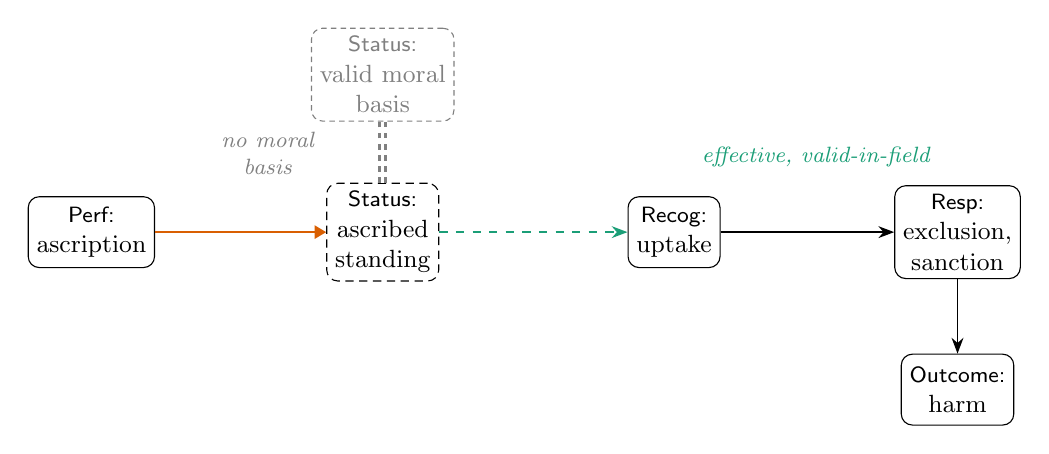
\begin{tikzpicture}
    \node[kind]    (u) at (0,0)    {\Nd{Perf}{ascription}};
    \node[flagged] (o) at (3.7,0)  {\Nd{Status}{ascribed\\standing}};
    \node[ghost]   (k) at (3.7,2)  {\Nd{Status}{valid moral\\basis}};
    \node[kind]    (r) at (7.4,0)  {\Nd{Recog}{uptake}};
    \node[kind]    (d) at (11.0,0) {\Nd{Resp}{exclusion,\\sanction}};
    \node[kind]    (l) at (11.0,-2) {\Nd{Outcome}{harm}};
    \draw[ntrans] (u) -- (o);
    \draw[recog]  (o) -- (r);
    \draw[causal] (r) -- (d);
    \draw[void]   (o) -- (k);
    \draw[causal] (d) -- (l);
    \node[font=\footnotesize\itshape, gray, align=center, anchor=east] at (2.95,1.0) {no moral\\basis};
    \node[font=\footnotesize\itshape, xGreen, anchor=south] at (9.2,0.7) {effective, valid-in-field};
  \end{tikzpicture}}
  \caption{Wrongful conferral. An ascribed standing is generated, recognized, taken up, and causally drives exclusion, sanction, and downstream harm, the recognitional and causal edges all live and the standing perhaps valid by the field's rules, while lacking a valid moral basis (grey, dashed). This is not the false-promise case, where recognition fails to fit an absent status, but a real conferred standing without moral warrant. Edge styles as in Figure~\ref{fig:promise}.}
  \label{fig:misrecognition}
\end{figure}

Discrimination is that regime case, and it shows the coupling at its sharpest. The efficacy is measurable, if crudely. In \textcite[997--998]{bertrandMullainathan2004EmilyGreg}'s correspondence study, otherwise-matched resumes with White-sounding names drew about 50\% more callbacks than those with African-American-sounding names (9.65\% against 6.45\%), and \textcite{ayres1991FairDriving} found parallel differential treatment in retail car negotiations. But such studies measure patterned uptake, not the metaphysics of the kind, and I lean on them only for that.

And in that limited sense, the recognitional pathway fires hard and projectibly: a raced signifier moves recognition, and recognition moves outcomes. A normative taxonomy with no place for this efficacy can't describe what's happening.

What do the audit studies actually manipulate? Not race, as \textcite{weinbergerSignalManipulation} observes, but a \emph{signal} for it: the name matters only because it reliably tracks race, and the experiment varies the signal to mimic what it would be were the candidate of another race, leaving the candidate's race untouched.

This is a legitimate, localized causal test of the signal-recognition-response pathway, just the recognitional and causal edges of the network. It neither makes race an ordinary manipulable cause nor concedes that causal analysis is impossible: the category is a distinct node, a conferred status the signal points to, not reducible to its signals.

But detection isn't discrimination. \textcite{kohlerHausmann2019EddieMurphy} is right that a signal test can show race made a difference without saying what race is or why discriminating on it is wrong; to read the test as defining discrimination is to mistake a proxy for a constituted social status, and \term{discrimination} is a thick concept that describes and condemns at once. \textcite{huForthcomingNormativeFactsCausalStructure} presses further: deciding which differences between two candidates constitute rather than confound the effect of race already takes a normative stand, so even the measurement presupposes the normative layer.

So discrimination is neither a causal regularity that happens to be wrong nor a normative verdict with sociological side effects. It's entrenched wrongful conferral: recognitional and causal edges firing reliably enough to be projectible, fixing a degraded standing that a field's rules may even license but morality doesn't.

This is why the recognition signature of Section~\ref{sec:coupling} matters most, holding the status fixed while recognition varies. Only a coupled, typed structure registers that the recognition is real and effective while the standing is morally void, whatever its standing in law, and so explains how an indefensible assignment becomes socially real without becoming just.

\section{Fields}
\label{sec:fields}

A field fixes the parameters the model so far leaves open: the status repertoire, the conditions under which each status is validly generated, which agents are authorized to confer or alter one, the channels recognition runs through and the threshold at which it counts, which records are kept, what responses and remedies a breach licenses, and what defeats a status.

In interpersonal morality breach projects toward blame, apology, repair, and trust revision; in contract law toward liability, damages, or excuse \citep{americanLawInstitute1981RestatementContracts}; in medicine toward authorization, protocol, and liability; in speech-act practice an illocutionary act alters the deontic-modal position of participants \citep{sbisa2023OnIllocutionaryTypes}.

Fields don't license arbitrary projections; they parameterize one shared typed network, which is how the account steers between universalism and relativism. (I use \enquote{field} loosely, for a normative setting or practice, not in Bourdieu's technical sense.) What sets a field's parameters is a further question: in \textcite{epstein2015AntTrap}'s terms, the frame principles that fix a status's grounding conditions are themselves anchored, and what anchors them need not be what any participant currently recognizes, so a field's rules don't reduce to current uptake.

Fields come in at least two kinds. An institutional field assigns status functions by authorized conferral; \textcite{searle1995Construction} builds these from the assignment of function, collective intentionality, and constitutive rules, and they carry deontic powers within a context. A contract, a diagnosis, a judgment, an accepted resignation live here, and so does authorized recognition. By contrast \textcite{asta2018Categories} marks out communal statuses, conferred by a community with the standing to confer but by no one in authority, gender and race among them.

This is why official judgment and discrimination, though both turn on recognition, behave so differently. The first is institutional: a recognition the field has authorized to make the status it records. The second is communal: a diffuse conferral with real constraints and enablements but no authorizing office, which is just why its standing can be socially effective while morally void. The field-type fixes which recognitions are status-altering and which are mere uptake.

\section{Conclusion}
\label{sec:conclusion}

The puzzle was that a status-assignment can be socially effective, and sometimes field-valid, without moral warrant. The answer is that some social and moral classifications are projectible only as nodes in a coupled, typed structure, with causal, normative-transition, and recognitional directed edges running within constitutive ties, and no one of these relation-types reduces to the others without losing the phenomenon. But causal regularity alone can't say why the wrongly-hounded man is wronged; normative status alone can't say why his being hounded is real.

This extends rather than overturns the causal-network account of kinds. Khalidi was right that projection needs order, not concatenation; the moral and institutional cases show that the order can be carried by non-causal edges and still support projection. What the coupled structure makes room for is a set of separations: efficacy from validity, and field-validity from moral warrant. Those are what let the apparatus describe misrecognition, and at regime scale the standing that oppressive law renders effective and even institutionally valid while leaving it morally void.

The strong claim isn't that some networks happen to contain both causal and normative relations, but that some explanations are unavailable unless the two are represented together. Where the boundaries of a field fall, whose recognition is authorized within it, and which misrecognitions harden into regimes are questions the framework poses rather than settles. That's where the next work lies.

\section*{Acknowledgements}

% TODO: Replace with the actual models used on this project and their current versions.
% Check model names: frontier models change frequently.
This paper was drafted with the assistance of large language models. All content has been reviewed and revised by the author, who takes full responsibility for the final text.

\newpage
\printbibliography

\end{document}
